\documentclass[11pt]{article}

\usepackage[utf8]{inputenc}
\usepackage[T1]{fontenc}

\usepackage{fullpage}

\usepackage{graphicx}
\usepackage{verbatim}
\usepackage{siunitx}

\usepackage[colorlinks=false,pdfborder={0 0 0}]{hyperref}
\usepackage[all]{hypcap}


\title{Astro 585: HW 2}
\author{Codename: The Maxwell-Jüttner Distribution}



\begin{document}


\maketitle

\section{Common Function Benchmarks}
\verbatiminput{1_common_benchmarks.jl}
Output:
\begin{verbatim}
rand: 5.467883391743815
.+:   0.7936923566738714
.*:   4.939859409921642
./:   2.0617212118723063
log:  0.7198937420711083
log10:0.7597877616464493
sin:  1.432453479819846
cos:  1.3486920641287916
tan:  0.670428735951879
atan: 0.7613800558965796
\end{verbatim}


\section{More Benchmarking}
Figure of time versus number of times executed is a the end of the section.
\verbatiminput{2_benchmark.jl}
Time versus number of times executed:
\begin{center}
	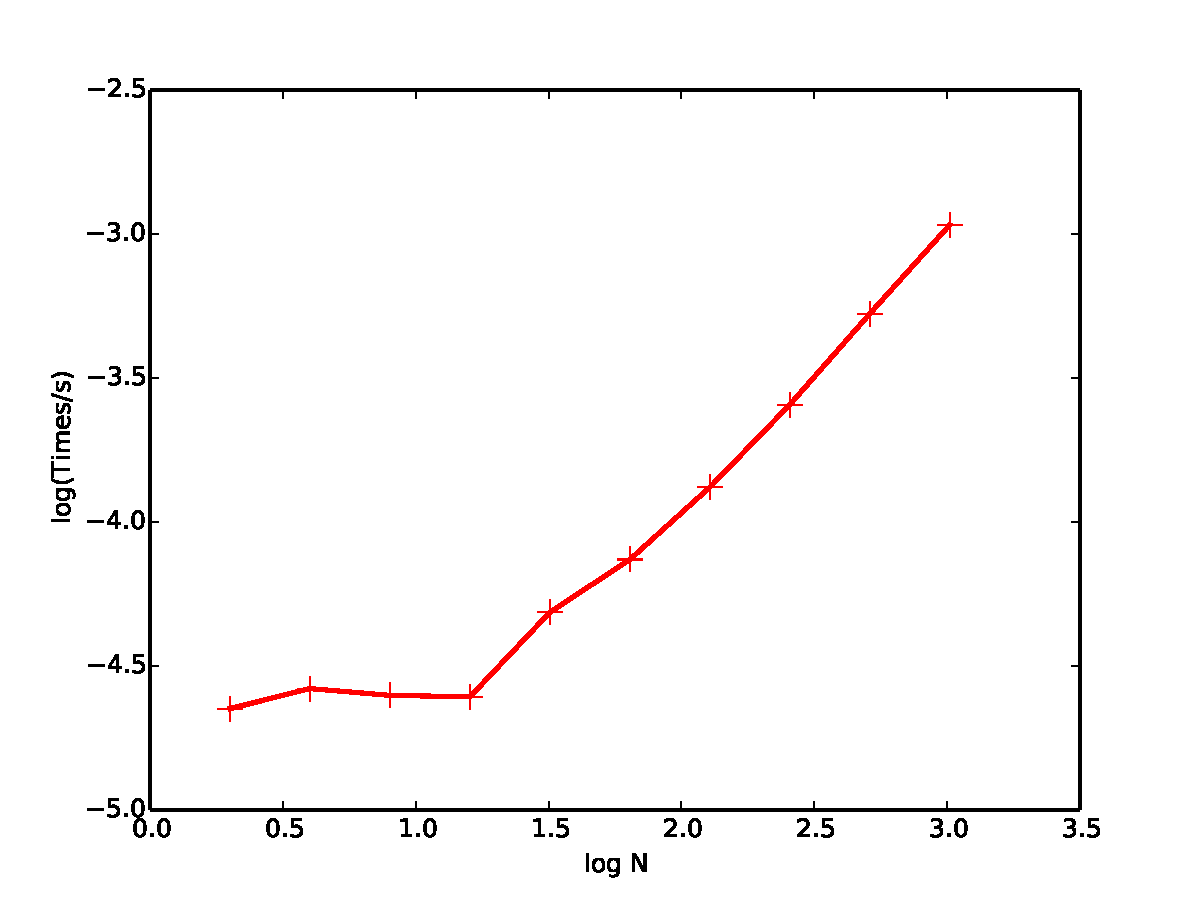
\includegraphics[width=0.5\textwidth]{benchmark.pdf}
\end{center}

\section{Euler Leapfrog}
\verbatiminput{3_integration.jl}
Using Euler's method:
\begin{center}
	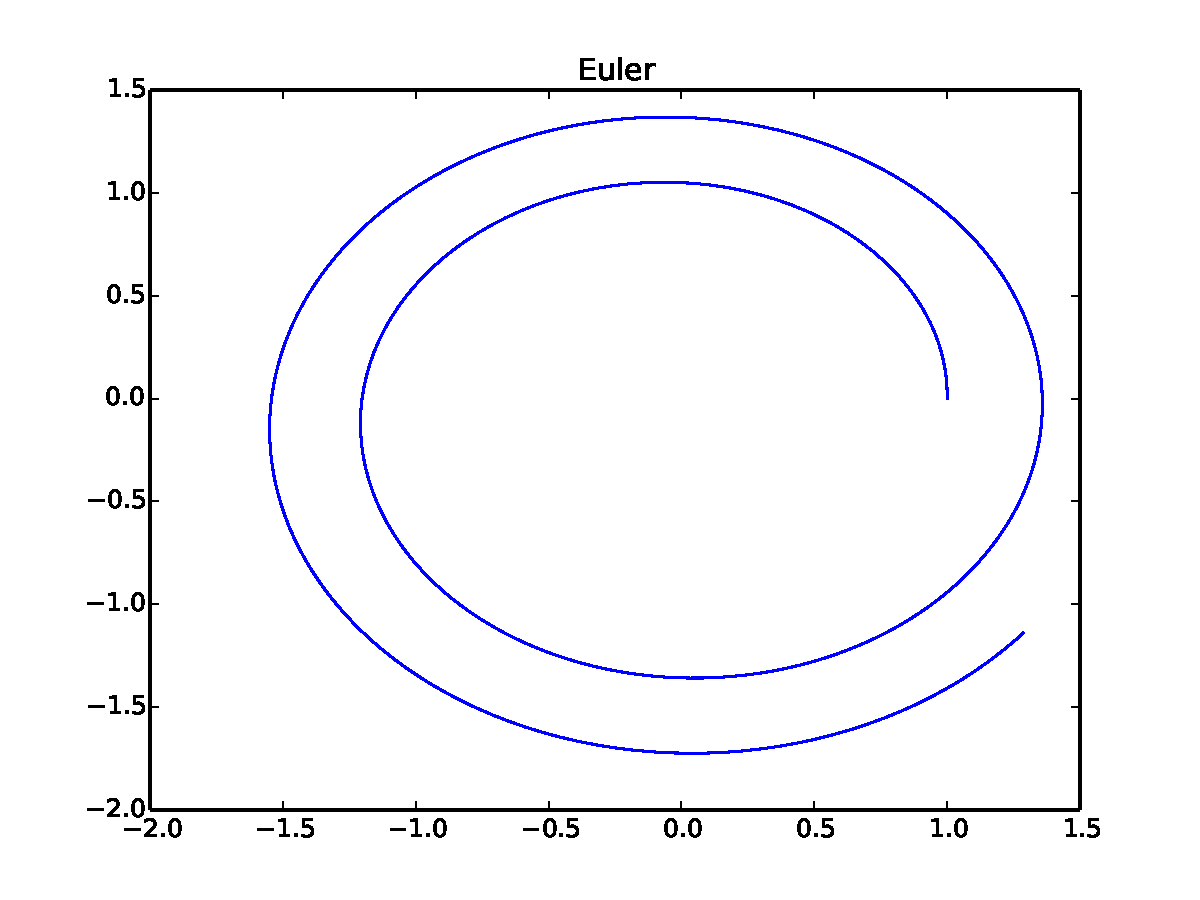
\includegraphics[width=0.45\textwidth]{euler.pdf}
\end{center}
Using the leapfrog method:
\begin{center}
	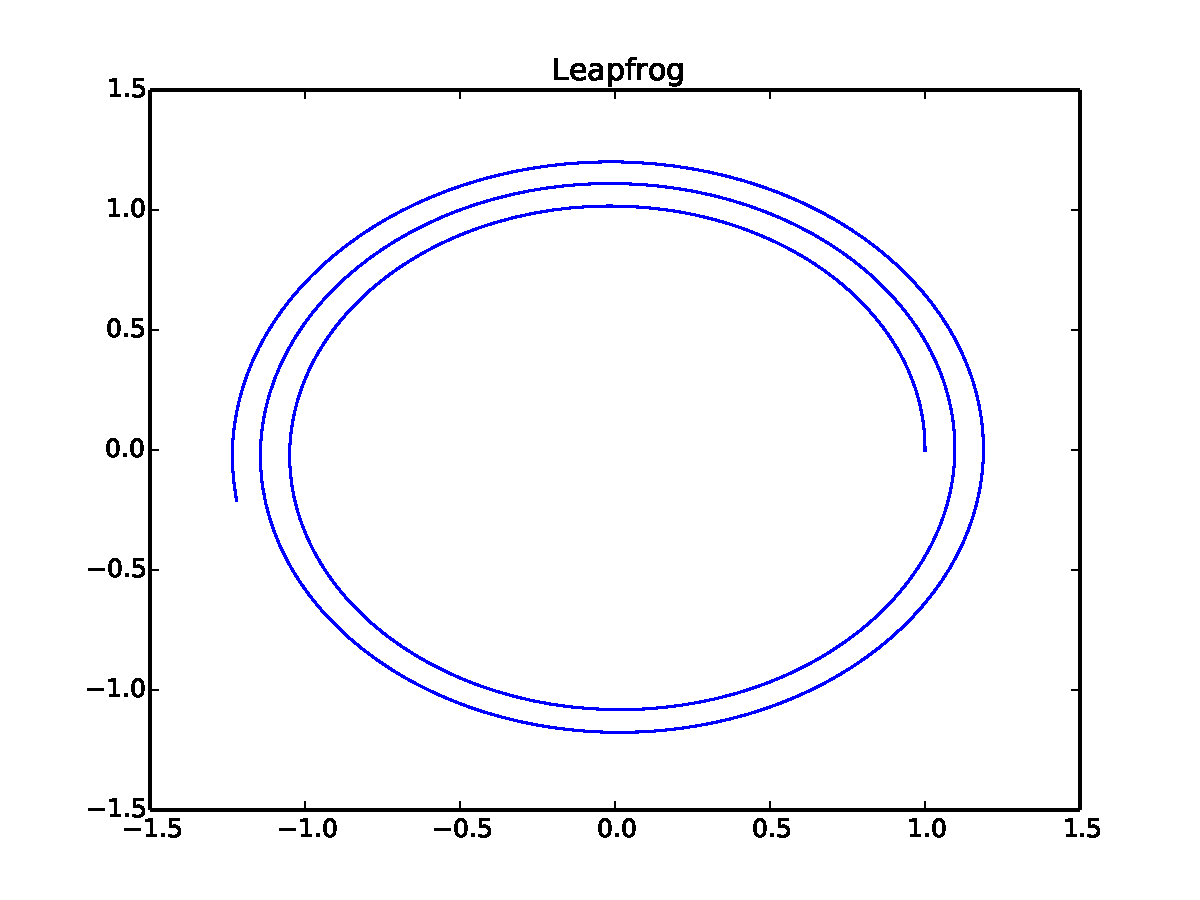
\includegraphics[width=0.45\textwidth]{leapfrog.pdf}
	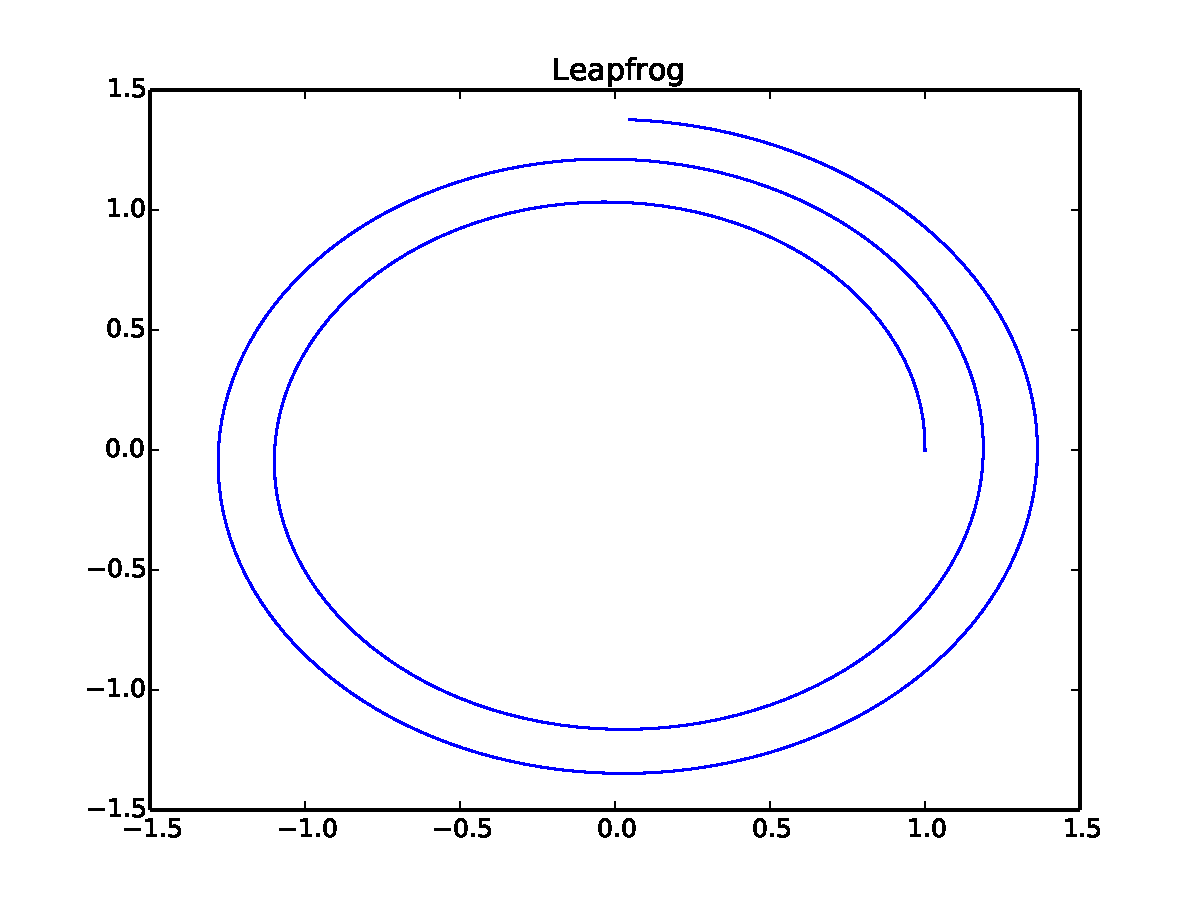
\includegraphics[width=0.45\textwidth]{leapfrog_bad.pdf}
\end{center}

\section{Memory and Speed}

\paragraph{4a)} Memory is $2^{32}$ bytes, size of one float is $2^3$ bytes, so
maximum is $2^{29}=5.36870912\times{}10^8$floats, so largest matrix would be
any rectangular one with that many entries, such as $2^{14}\times{}2^{15}$. The
largest square matrix would be $23170\times{}23170$, with a few bytes (176096
bytes) to spare for the program, and possibly an operating system\ldots

\paragraph{4b)}
$$ n = 23170 $$
Number of computations needed is
$$ m = \frac{2}{3} n^3 = \num{8.29e12} $$
Time is approximately
$$ t = \frac{m}{r} = \frac{\num{8.29e12}}{\SI{20e9}{flops\per\second}} = \SI{414.6263004333333}{\second} $$
A few minutes.

\paragraph{4c)} Memory seems to be a more stringent constraint, although I am
not so sure that \SI{20}{\giga{}flops\per\second} is so realistic unless there
is significant parallelization. Also, the floats need to be transferred from
the memory to the CPU and back, which is likely going to be much slower than
the \SI{20}{\giga{}flops\per\second}.

\paragraph{4d)} The phase of the Moon!

\paragraph{4e)} One could come up with an algorithm that operates only on parts
of the original matrix at a time, such as splitting the matrix into blocks such
that a few blocks fit into memory. Blocks that are not needed could be stored
on disk, or on other nodes in a cluster. Either one will introduce extra
overhead reading from disk or transferring blocks from one node to another.


\end{document}
